\documentclass[12pt, letterpaper]{article}
\usepackage[utf8]{inputenc}
\usepackage{geometry}
\geometry{margin=1in}
\usepackage{graphicx}
\usepackage{float}
\usepackage{booktabs}
\usepackage{amsmath}
\usepackage{caption}
\usepackage{subcaption}
\usepackage{xcolor}
\usepackage{tcolorbox}
\usepackage{tikz}
\usetikzlibrary{shapes, arrows, positioning, calc, decorations.pathmorphing, shadows}
\usepackage{circuitikz} % Try to use if available, otherwise fallback to tikz
\usepackage{listings}
\usepackage{array}
\usepackage{titlesec}
\usepackage{fancyhdr}
\usepackage{hyperref}
\usepackage[nameinlink,noabbrev]{cleveref}

% --- Caption formatting ---
\captionsetup{
  font=small,
  labelfont=bf,
  labelsep=period,
  justification=centering,
  singlelinecheck=false,
  skip=6pt
}
\captionsetup[table]{position=top}

% --- Section headings ---
\titleformat{\section}{\Large\sffamily\bfseries}{\thesection}{0.6em}{}
\titleformat{\subsection}{\large\sffamily\bfseries}{\thesubsection}{0.5em}{}
\titleformat{\paragraph}[block]{\normalfont\normalsize\bfseries}{}{}{}
\titlespacing*{\section}{0pt}{1.2ex plus .3ex}{0.6ex}
\titlespacing*{\subsection}{0pt}{1.0ex plus .2ex}{0.4ex}
\titlespacing*{\paragraph}{0pt}{0.8ex}{0.6ex}

% --- Header / footer ---
\newcommand{\coursenum}{MECH 421}
\newcommand{\labnum}{Lab 5}
\newcommand{\labtitle}{PCB Assembly and Stepper Motor Control}
\newcommand{\studentone}{Gyan Edbert Zesiro}
\newcommand{\studentoneid}{38600060}
\newcommand{\studenttwo}{Ryan Edric Nashota}
\newcommand{\studenttwoid}{33508219}
\newcommand{\labperformed}{7~November~2025}
\newcommand{\labsubmitted}{28~November~2025}
\pagestyle{fancy}
\fancyhf{}
\lhead{\sffamily \labnum}
\chead{\sffamily \labtitle}
\rhead{\sffamily Gyan, Ryan}
\renewcommand{\headrulewidth}{0.4pt}
\cfoot{\sffamily \thepage}
\setlength{\headheight}{15pt}
\addtolength{\topmargin}{-3pt}

% --- Cleveref ---
\Crefname{figure}{Figure}{Figures}
\Crefname{table}{Table}{Tables}
\Crefname{equation}{Equation}{Equations}
\Crefname{section}{Section}{Sections}
\crefname{figure}{figure}{figures}
\crefname{table}{table}{tables}
\crefname{equation}{equation}{equations}
\crefname{section}{section}{sections}

% --- Graphics path ---
\graphicspath{{../analysis_outputs/figures/}{figures/}}
\newtcolorbox{infobox}[1][]{colback=blue!5,colframe=cyan!60!black,title=#1,boxrule=0.6pt}

% --- Code listing style ---
\definecolor{codegreen}{rgb}{0,0.6,0}
\definecolor{codegray}{rgb}{0.5,0.5,0.5}
\definecolor{codepurple}{rgb}{0.58,0,0.82}
\definecolor{backcolour}{rgb}{0.95,0.95,0.92}

\lstdefinestyle{mystyle}{
    backgroundcolor=\color{backcolour},
    commentstyle=\color{codegreen},
    keywordstyle=\color{magenta},
    numberstyle=\tiny\color{codegray},
    stringstyle=\color{codepurple},
    basicstyle=\ttfamily\footnotesize,
    breakatwhitespace=false,
    breaklines=true,
    captionpos=b,
    keepspaces=true,
    numbers=left,
    numbersep=5pt,
    showspaces=false,
    showstringspaces=false,
    showtabs=false,
    tabsize=2
}
\lstset{style=mystyle}

% --- Placeholder command for images ---
\newcommand{\imageplaceholder}[2]{
    \begin{figure}[H]
        \centering
        \fbox{\begin{minipage}{0.8\textwidth}
            \centering
            \vspace{2cm}
            \textbf{PLACEHOLDER FOR: #1} \\
            \vspace{1cm}
            \textit{#2}
            \vspace{2cm}
        \end{minipage}}
        \caption{#1}
        \label{fig:#1}
    \end{figure}
}

% --- Title block ---
\makeatletter
\renewcommand{\maketitle}{
  \vspace*{1ex}
  \begin{center}
    {\sffamily
      {\Large \coursenum\ --- \labnum\par}
      \vspace{0.6ex}
      {\huge \bfseries \labtitle\par}
      \vspace{0.8ex}
      {\large \studentone\enspace (ID:\ \studentoneid) \\[0.4ex]
      \studenttwo\enspace (ID:\ \studenttwoid)\par}
      \vspace{0.6ex}
      {\normalsize  Report Submitted:\ \labsubmitted\par}
    }
  \end{center}
  \vspace{1.2ex}
  \thispagestyle{empty}
}
\makeatother

% --- Body spacing ---
\setlength{\parindent}{0pt}
\setlength{\parskip}{0.6em}

% --- Metadata ---
\title{\coursenum\ \labnum\\\labtitle}
\author{\studentone\ (ID:\ \studentoneid) \\ \studenttwo\ (ID:\ \studenttwoid)}
\date{}

\begin{document}
\pagenumbering{gobble}
\maketitle

\begin{abstract}
This lab focused on building and testing a PCB designed to control stepper, and DC motors
through microprocessor commands, though for this lab we are only focusing on 
stepper motors. The lab was completed in three main sections. 
First, we assembled and soldered the PCB, verifying proper functionality of the power supply, USB interface, microprocessor, 
and motor driver components. We configured UART communication to enable data transfer for 
future exercises. Second, we developed firmware to control a stepper motor using half-stepping, 
implementing both single-step commands and continuous velocity control through a C\# graphical interface. 
We expanded the system to control a two-axis gantry stage using dual stepper motors. We programmed the microcontroller 
to execute coordinated movements, allowing the stage to follow straight-line paths between specified coordinates. 
The system successfully drew predetermined shapes and a custom design, demonstrating precise synchronized control of both axes. 
Throughout the lab, we gained practical experience in PCB assembly, firmware development, serial communication protocols, 
and motion control algorithms while exploring the advantages and limitations of stepper motors for precision positioning applications.
\end{abstract}

\clearpage
\pagenumbering{roman}
\setcounter{page}{1}
\renewcommand{\contentsname}{Table of Contents}
\tableofcontents
\clearpage
\renewcommand{\listfigurename}{Table of Figures}
\listoffigures
\clearpage
\listoftables
\clearpage
\setcounter{tocdepth}{2}
\pagenumbering{arabic}
\setcounter{page}{1}
\pagestyle{fancy}

\section{Introduction}
The purpose of this lab is to gain hands-on experience in PCB assembly, soldering surface-mount components, and 
implementing real-time control for stepper motors using a microcontroller. 
The final system is a 2-axis gantry capable of drawing complex shapes, demonstrating the integration of hardware 
(PCB, motors, mechanics) and software (firmware, PC interface).

\section{Exercise 1: PCB Assembly and Soldering}

\subsection{Objective}
The goal of this exercise is to populate a bare PCB with surface-mount and through-hole components to create a 
functional motor control board. This board includes a microcontroller (MSP430), USB interface (FTDI), power regulation, 
and motor drivers. This exercise also teaches us how to solder SMD components and troubleshoot common issues.

\subsection{Circuit Description}
The PCB consists of several key functional blocks:
\begin{itemize}
    \item \textbf{Power Supply}: Converts external 12V DC input to 5V and 3.3V logic levels using linear regulators (NCP1117). 5V is used for the USB interface and some logic, while 3.3V powers the MSP430 microcontroller.
    \item \textbf{USB Interface}: Uses an FT230XS chip to convert USB signals from a PC into UART (Serial) signals compatible with the microcontroller. This allows for data logging and control commands.
    \item \textbf{Microcontroller}: The MSP430FR5739 is the brain of the board. It executes firmware to generate PWM signals for motors, read sensors, and communicate via UART.
    \item \textbf{Motor Driver}: The DRV8841 is a dual H-bridge driver capable of driving DC motors or bipolar stepper motors. It handles the high currents required by the motors, controlled by low-power logic signals from the MCU.
\end{itemize}

\subsection{Parts List}
The following components are required for assembly. Ensure all parts are accounted for before starting.

\begin{table}[H]
\centering
\begin{tabular}{@{}>{\raggedright\arraybackslash}p{4.6cm}%
                >{\raggedright\arraybackslash}p{6.7cm}%
                >{\centering\arraybackslash}p{1.5cm}%
                >{\centering\arraybackslash}p{1.0cm}@{}}
\toprule
\textbf{Reference} & \textbf{Description} & \textbf{Source} & \textbf{Qty} \\ \midrule
5x1 header programming & Bergstik II 0.100" straight header & Kit & 1 \\
Motor bypass cap & 1000\,$\mu$F 50V 20\% alum SMD & Kit & 2 \\
MCU core bypass & 0.47\,$\mu$F 16V 5\% X7R 0603 & Kit & 1 \\
0.01\,$\mu$F charge pump critical & 10{,}000\,pF 100V 5\% NP0 1206 & Kit & 1 \\
51\,pF filter encoder & 51\,pF 50V 5\% NP0 1206 & Kit & 2 \\
20-pin MCU header & 20\,pos 0.100" straight header & Kit & 2 \\
DC wall jack & 2.1\,mm PCB power jack & Kit & 1 \\
USB connector & Mini-USB receptacle, 5\,pos & Kit & 1 \\
PSU diode & Schottky diode 40V 3A DO-214AC & Kit & 2 \\
Polyfuse USB & Resettable fuse 6V 0.50A 1206 & Kit & 1 \\
Latch & Dual D-type latch, 14-SOIC & Kit & 2 \\
Inverter & Hex Schmitt-trigger inverter, 14-SOIC & Kit & 2 \\
3.3V PSU & LDO regulator 3.3V 1A SOT-223 & Kit & 1 \\
5.0V PSU & LDO regulator 5V 1A SOT-223 & Kit & 1 \\
USB chip (FT230XS) & USB serial basic UART 16-SSOP & Kit & 1 \\
Green LED & Green LED clear 1206 SMD & Kit & 6 \\
Current sense resistors & 0.2\,$\Omega$ 2W 1\% 2512 & Kit & 2 \\
1.0\,k$\Omega$ (Replace B) & 1.0\,k$\Omega$ 1/4W 5\% 1206 SMD & Kit & 3 \\
2.7\,k$\Omega$ encoder pullup 1\% & 2.7\,k$\Omega$ 1/4W 1\% 1206 SMD & Kit & 4 \\
27\,$\Omega$ USB terminal 1\% & 27\,$\Omega$ 1/4W 1\% 1206 SMD & Kit & 2 \\
30\,k$\Omega$ driver pullups & 30\,k$\Omega$ 1/4W 5\% 1206 SMD & Kit & 2 \\
3.0\,k$\Omega$ bypass resistors & 3\,k$\Omega$ 1/4W 5\% 1206 SMD & Kit & 4 \\
47\,k$\Omega$ programming pullup & 47\,k$\Omega$ 1/4W 5\% 1206 SMD & Kit & 1 \\
Crystal & 24.00\,MHz resonator with caps, SMD & Kit & 1 \\
Screw terminal & 5.08\,mm vertical terminal block, 2-pos & Kit & 4 \\
Bypass general & 0.1\,$\mu$F 100V 10\% X7R 1206 & Lab & 18 \\
PSU bypass (Replace A) & 4.7\,$\mu$F 50V 10\% X7R 1206 & Lab & 8 \\
Current limiting resistors & 150\,$\Omega$ 1/10W 5\% 0603 SMD & Lab & 42 \\
4x1 header (opt) & 4\,pos 0.100" straight header & Optional & 3 \\
XBee socket (opt) & 10\,pos 2\,mm vertical socket & Optional & 1 \\
Test point (opt) & Mini 0.040" OD black test point & Optional & 10 \\
PSU bypass & 10\,$\mu$F 50V 20\% X5R 1206 & Replace A & 8 \\
2.4\,k$\Omega$ driver LED (24VDC max) & 2.4\,k$\Omega$ 1/4W 5\% 1206 SMD & Replace B & 2 \\
330\,$\Omega$ 3.3V LED power & 330\,$\Omega$ 1/4W 5\% 1206 SMD & Replace B & 2 \\
510\,$\Omega$ 5V LED power & 510\,$\Omega$ 1/4W 5\% 1206 SMD & Replace B & 2 \\
MCU & 16-bit MCU, 16KB FRAM, 38-TSSOP & Kit & 1 \\
Motor controller & Motor driver, 28-HTSSOP & Kit & 1 \\
\bottomrule
\end{tabular}
\caption{Complete components list for PCB assembly}
\end{table}

\subsection{SMD and Through-Hole Soldering Techniques}
Before commencing the full assembly, we established a standardized workflow for soldering the various component types. While hot air rework is effective for SMD parts with thermal pads, we completed the build with a fine-point soldering iron to maintain manual control.

The key enabler was flux. The kit's flux pen was okay for this lab soldering, but we had much better success with liquid flux 
from a syringe, which improved solder flow and reduced bridging. Most of the soldering techniques can be found in this linked video,
\noindent \textbf{Video}: \href{https://youtu.be/fYInlAmPnGo?si=vKOG1YNxM5TwRe-x}{SMD Soldering Tutorial (YouTube)}


\subsubsection{Passive Components (0603 Resistors and Capacitors)}
For small two-terminal parts we used a tack-and-reflow method:
\begin{enumerate}
    \item Tin a single pad with a small solder dot.
    \item Hold the component with tweezers, reflow the tinned pad, and slide the part into place.
    \item Confirm it is flat; then solder the second pad.
\end{enumerate}


\subsubsection{Integrated Circuits (Fine-Pitch ICs)}
We used a pin-by-pin transfer to reduce bridges:
\begin{enumerate}
    \item Align the chip and tack one corner pin.
    \item Flood pins with liquid flux.
    \item Place a small solder blob on the iron tip and touch each pin/pad junction; flux pulls solder onto the joint without bridging.
    \item Clear any excess with copper braid.
\end{enumerate}


\subsubsection{Through-Hole Components}
For connectors (USB, JTAG, DC jack):
\begin{enumerate}
    \item Insert leads and secure by bending or taping.
    \item Heat pad and lead together; feed solder into the joint until a small cone forms.
    \item Remove solder, then iron, and let cool undisturbed.
\end{enumerate}
\noindent \textbf{Video}: \href{https://www.youtube.com/watch?v=IpkkfK937mU}{How to Solder Through-Hole Components (YouTube)}

\subsubsection{Note on Hot Air Reflow}
Though not necessary, we looked around YouTube and found that
potentially using solder paste and hot air gun can be easier for SMD soldering. 
This technique can self-align parts via surface tension and should speed up the soldering process, especially for ICs.
\noindent \textbf{Video}: \href{https://www.youtube.com/shorts/vk-QlYruoko}{Soldering with Heatgun and Solder Paste (YouTube)}

\subsection{Assembly Procedure}
The assembly was performed in the following sequence, testing each stage before proceeding:

\subsubsection{Step 1: Underside Resistors}
We began by soldering the 150 $\Omega$ current-limiting resistors on the bottom side. These 0603 parts also warmed us up for the finer SMD work.
\begin{itemize}
    \item Tack-and-reflow (tin one pad, place with tweezers, reflow, then solder the second pad).
    \item For checking, measure across each resistor footprint with a multimeter; expect $\approx$150 $\Omega$ per resistor.
\end{itemize}

\subsubsection{Step 2: Power Supply}
The power supply section converts the 12V input to 5V and 3.3V rails.
\begin{itemize}
    \item Solder the following components, DC Jack, LED, S34 diodes (polarity critical), NCP1117 regulators, tantalum/ceramic capacitors.
    \item For the diodes make sure that the cathode (marked end) aligns with the silkscreen bar.
    \item For LEDs, ensure correct orientation.
    \item To verify the system, connect to a 12V power supply. The power LED should glow brightly at 12V. Additionally, measure $\approx$5.0V and $\approx$3.3V on the regulators' outputs.
\end{itemize}
See \Cref{fig:power-supply-layout,fig:power-supply-schematic} for layout and schematic reference.
\begin{figure}[H]
  \centering
  \begin{subfigure}[b]{0.45\textwidth}
    \includegraphics[width=\textwidth]{figures/power_supply_layout.png}
    \caption{Power supply PCB layout}
    \label{fig:power-supply-layout}
  \end{subfigure}\hfill
  \begin{subfigure}[b]{0.45\textwidth}
    \includegraphics[width=\textwidth]{figures/power_supply_schematic.png}
    \caption{Power supply schematic}
    \label{fig:power-supply-schematic}
  \end{subfigure}
  \caption{Power supply reference during assembly}
\end{figure}

\subsubsection{Step 3: USB Interface}
This section enables communication with the PC.
\begin{itemize}
    \item Solder the following components, FT230XS (SSOP-16), Mini-USB connector, protection circuitry.
    \item For the IC and USB use continuity checks to ensure no bridges between pins.
    \item The last 2 pins on the Mini-USB connector are not connected as such they might make a sound in continuity test, however rest assured
    that they will still work.
    \item \textbf{Solution}: We used flux and desoldering braid to potential bridges.
    \item To verify, plug into a PC; listen for the USB connect chime and confirm the device enumerates as "USB Serial Port (COM3)". 
    The FT230XS should stay cool to the touch (no noticeable heating).
\end{itemize}
See \Cref{fig:usb-layout,fig:usb-schematic} for the USB layout and schematic.
\begin{figure}[H]
  \centering
  \begin{subfigure}[b]{0.48\textwidth}
    \includegraphics[width=\textwidth]{figures/usb_layout.png}
    \caption{USB interface PCB layout}
    \label{fig:usb-layout}
  \end{subfigure}\hfill
  \begin{subfigure}[b]{0.48\textwidth}
    \includegraphics[width=\textwidth]{figures/usb_schematic.png}
    \caption{USB interface schematic}
    \label{fig:usb-schematic}
  \end{subfigure}
  \caption{USB interface reference during assembly}
\end{figure}

\subsubsection{Step 4: Microcontroller}
The core of the system.
\begin{itemize}
    \item Solder the following components, MSP430FR5739 (TSSOP-38), 24MHz crystal oscillator, JTAG header.
    \item We find it easier to solder the MCU first and then the crystal, so that the crystal won't block the angle of solder for some of the IC pins.
    \item For the crystal, there are 3 pads, you can do the tack and reflow technique on one pad, then solder the other two pads normally.
    \item To verify the circuit works, we flashed a simple LED blink for the MSP430 via CCS; the blinking LED confirms JTAG wiring and basic MCU operation.
\end{itemize}
See \Cref{fig:mcu-layout} for the MSP430 placement and decoupling.
\begin{figure}[H]
  \centering
  \includegraphics[width=0.8\textwidth]{figures/mcu_layout.png}
  \caption{MSP430FR5739 layout reference}
  \label{fig:mcu-layout}
\end{figure}

\subsubsection{Step 5: Motor Driver and Encoder}
Finally, the high-power motor drivers and encoder logic were added.
\begin{itemize}
    \item Solder,  DRV8841 (HTSSOP-28), 74HC14/74 connections.
    \item For the motor driver, ensure that the thermal pad is soldered via the back. This provides the necessary function for heat dissipation as the
    driver will be very hot otherwise.
    \item You can verify this by using UART to communicate with device, then run a 
    firmware routine to toggle the motor driver outputs and observe signals on the motor pins.
    \item The encoder section has not yet been tested in this lab as it will be used for future MECH423 labs, however we can still 
    verify continuity on the encoder pins to ensure no shorts.
\end{itemize}
See \Cref{fig:motor-driver-layout,fig:shaft-encoder-layout} for driver and encoder routing.
\begin{figure}[H]
  \centering
  \includegraphics[width=0.8\textwidth]{figures/motor_driver_layout.png}
  \caption{Motor driver layout reference}
  \label{fig:motor-driver-layout}
\end{figure}

\begin{figure}[H]
  \centering
  \includegraphics[width=0.8\textwidth]{figures/shaft_encoder_layout.png}
  \caption{Shaft encoder layout reference}
  \label{fig:shaft-encoder-layout}
\end{figure}

\subsection{Results and Discussion}
\begin{figure}[H]
  \centering
  \includegraphics[width=0.8\textwidth]{figures/pcb_board_front.jpeg}
  \caption{Assembled PCB (Front)}
  \label{fig:ex2-pcb-front}
\end{figure}
\begin{figure}[H]
  \centering
  \includegraphics[width=0.8\textwidth]{figures/pcb_board_back_overview.jpeg}
  \caption{Assembled PCB (Back)}
  \label{fig:ex2-pcb-back}
\end{figure}

\subsection{Challenges} 
\begin{enumerate}
    \item Early joints on resistors/capacitors/LEDs worked electrically but looked rough; practice improved finish. One pad lifted when we overused the vacuum pump, but we repaired the net with a wire jumper.
    \item Fine-pitch IC pins were hard to see; a magnifying glass was essential to spot bridges.
    \item A solder bridge between pins 15 and 16 of the FT230XS blocked USB enumeration. We cleared it with braid plus liquid flux and cleaned with IPA; USB then enumerated.
    \item Fine pitch IC's can be hard to solder
    \item A smaller-nozzle, temperature-controlled hot air tool would reduce collateral heat when reworking ICs; thick solder wire also made control harder, so thinner wire or solder paste would be better for future IC work.
    \item The iron tip felt oversized at times; smaller tips plus paste would speed IC soldering and reduce errors.
    \item The DRV8841 driver got very hot when powered without a motor load. We limited PWM duty cycle in firmware to reduce heating.
\end{enumerate}

\section{Exercise 2: Stepper Motor Control}

\subsection{Objective}
To control a bipolar stepper motor using the assembled PCB. This involves generating precise PWM waveforms to drive the motor phases in a specific sequence (half-stepping) and implementing a UART interface for velocity control.

\subsection{UI Computations and Telemetry}
\paragraph{Single-step.} Each press calls \texttt{MoveByAngle} with the half-step increment $\theta_{\text{step}} = 360^{\circ}/N_{\text{steps}}$ and wraps position with $p_{\text{deg}} = (\text{deg} \bmod 360 + 360) \bmod 360$ to stay in $[0,360)$.

\paragraph{Continuous mode.} The slider $s\in[-100,100]$ maps to signed steps/s, RPM, and TA1CCR0:
\begin{align}
  f_{\text{steps}} &= \max\!\bigl(1,\; |s|/100 \cdot f_{\text{max}}\bigr)\,\text{sgn}(s) \\
  \text{RPM} &= \frac{f_{\text{steps}}\cdot 60}{N_{\text{steps}}} \\
  \text{TA1CCR0} &= \frac{f_{\text{clk}}}{|f_{\text{steps}}|} - 1,\qquad f_{\text{clk}}=1{,}000{,}000~\text{Hz} \\
  f_{\text{step\_timer}} &= \frac{f_{\text{clk}}}{\text{TA1CCR0}+1}
\end{align}
where $N_{\text{steps}}=200$ (SY35ST36 motor) and $f_{\text{max}}$ comes from the UI numeric box (default 1200~steps/s). The code that applies these equations and sends the UART packet is shown in \Cref{lst:handle-velocity}.
\begin{lstlisting}[language=C, caption={Continuous mode mapping and packet send}, label={lst:handle-velocity}]
private void HandleVelocityChange()
{
    int sliderValue = velocityTrackBar.Value;          // s in [-100, 100]
    double maxStepsPerSecond = (double)maxSpeedNumeric.Value; // f_max
    if (sliderValue == 0) { StopMotor("Slider at zero -> stop timer"); return; }
    double fraction = Math.Abs(sliderValue) / 100.0;
    double commandedStepsPerSecond = Math.Max(1.0, fraction * maxStepsPerSecond);
    bool clockwise = sliderValue > 0;
    double rpm = commandedStepsPerSecond * 60.0 / StepperCommander.StepsPerRevolution;
    if (!clockwise) rpm *= -1;
    byte dir; ushort ccr0;
    byte[] packet = commander.BuildContinuousPacketFromRpm(rpm, out ccr0, out dir);
    commander.SendPacket(packet);
    UpdateVelocityLabels(sliderValue, commandedStepsPerSecond, ccr0);
    UpdateModeAndFreq($"Continuous {(clockwise ? "CW" : "CCW")}", ccr0);
    SetTelemetry(commander.CurrentAngleDeg, commandedStepsPerSecond);
}
\end{lstlisting}

\subsection{Stepper Motor Basics}
\subsubsection{Stepper Motor Operation}
The stepper motor has two coils (Phase A and Phase B). As seen in \Cref{fig:stepping}, by energizing these coils in a specific sequence, 
the rotor aligns with the magnetic field, moving in discrete steps.
\begin{itemize}
    \item \textbf{Full-Stepping}: Energizing phases in sequence (A+ $\rightarrow$ B+ $\rightarrow$ A- $\rightarrow$ B-).
    \item \textbf{Half-Stepping}: Inserting intermediate states where both phases are energized, doubling the resolution (A+ $\rightarrow$ A+B+ $\rightarrow$ B+ ...).
\end{itemize}

\begin{figure}
    \centering
    \includegraphics[width=0.6\textwidth]{figures/a-Full-step-operation-and-b-half-step-operation-for-a-two-phase-stepping-motor.png}
    \caption{Full and Half-stepping sequence for a bipolar stepper motor}
    \label{fig:stepping}
\end{figure}

We will use the half-stepping profile in our firmware to control the stepper motor. 

\subsubsection{Current Control (PWM)}
To prevent overheating, the voltage applied to the coils is modulated using Pulse Width Modulation (PWM). 
A duty cycle of roughly 25\% is sufficient for no-load operation.

\subsection{Firmware Implementation}
The firmware implements a lookup-based state machine to drive the stepper motor. 
To support variable speed, a Timer (TB0/TB1) is used to generate PWM signals for current control, 
while a periodic interrupt (Timer A1) advances the step state.

\subsubsection{Lookup Table}
The half-stepping sequence requires 8 distinct states. We used the following bitmask table where bits correspond to 
the phases A1, A2, B1, B2:

\begin{tcolorbox}[colback=green!5!white,colframe=green!75!black,title=Stepper Step Table]
\begin{lstlisting}[language=C, caption={Half-step lookup table}, label={lst:stepper-table}]
// Half-step lookup table (8 steps)
// bit0=A1, bit1=A2, bit2=B1, bit3=B2
static const uint8_t stepper_table[8] = {
    0b0001, // 1: A1
    0b0101, // 2: A1+B1
    0b0100, // 3: B1
    0b0110, // 4: B1+A2
    0b0010, // 5: A2
    0b1010, // 6: A2+B2
    0b1000, // 7: B2
    0b1001  // 8: B2+A1
};
\end{lstlisting}
\end{tcolorbox}

\subsubsection{Step Generation Logic}
The \texttt{step\_motor1} function applies these masks to the Timer Capture Compare Registers 
(TB0CCR1/2, TB1CCR1/2) to set the PWM duty cycle for each connected pin.

\begin{lstlisting}[language=C, caption={Step generation logic}, label={lst:step-motor1}]
void step_motor1(uint8_t step) {
    uint8_t mask = stepper_table[step & 0x07];
    // Update PWM Duty Cycles based on mask
    TB0CCR2 = (mask & 0x01) ? PWM_DUTY : 0; // A1
    TB0CCR1 = (mask & 0x02) ? PWM_DUTY : 0; // A2
    TB1CCR2 = (mask & 0x04) ? PWM_DUTY : 0; // B1
    TB1CCR1 = (mask & 0x08) ? PWM_DUTY : 0; // B2
}
\end{lstlisting}

\subsection{Comparison with DC Motor Control}
While this lab focused on stepper motors, the lab manual did mention DC motors for motion control. The key differences are:

\begin{itemize}
    \item \textbf{Control Loop}: Stepper motors primarily operate in an open-loop configuration (command steps = assumed position). DC motors require a closed-loop system with feedback (e.g., an encoder) to control position or velocity accurately.
    \item \textbf{Torque}: Steppers have high holding torque at low speeds but drop off at high speeds. DC motors maintain torque better across the speed range but require continuous power to hold position against a load (unless geared).
    \item \textbf{Resolution}: Stepper resolution is fixed by the step angle (1.8$^\circ$). DC motor resolution depends on the encoder PPR (Pulses Per Revolution).
\end{itemize}

Controlling the movement of a DC motor would require constantly changing the PWM to match the desired speed or position. 
As such, often to control a DC motor's position, a PID loop reading an encoder is required. The pseudocode for such a system would be:

\begin{lstlisting}[language=C, caption={DC motor PID pseudocode}, label={lst:dc-pid}]
// ISR triggered by Encoder Pulse
void Encoder_ISR() {
    if (ChannelA == ChannelB) position++;
    else position--;
}

// Control Loop (e.g., 100Hz Timer)
void Control_Loop() {
    error = target_pos - position;
    integral += error;
    derivative = error - prev_error;
    
    pwm_output = (Kp * error) + (Ki * integral) + (Kd * derivative);
    
    set_motor_pwm(pwm_output);
    prev_error = error;
}
\end{lstlisting}

\subsection{Software Interface (C\#)}
The C\# application acts as the commander. It sends packets to the MCU to set velocity or trigger single steps.
We programmed it to have two modes: single-step (half-step CW/CCW) and continuous velocity control (CW/CCW). 
The half-step buttons issue one table entry per press, update position telemetry, and stop the motor when requested. 
Continuous mode streams a signed speed derived from the slider and converts it to TA1CCR0. See \Cref{fig:ui-step,fig:ui-continuous} 
for both screens.
\begin{figure}[H]
  \centering
  \includegraphics[width=0.9\textwidth]{figures/ex2_ui_cont.png}
  \caption{Single-step UI: half-step CW/CCW buttons with stop and position telemetry}
  \label{fig:ui-step}
\end{figure}
\begin{figure}[H]
  \centering
  \includegraphics[width=0.9\textwidth]{figures/ex2_ui_step.png}
  \caption{Continuous UI: slider sets signed speed, TA1CCR0 is reported}
  \label{fig:ui-continuous}
\end{figure}

Packets follow the layout in \Cref{fig:packet-diagram} and feed the half-step table in \Cref{lst:stepper-table}. The start byte gates parsing; the instruction selects mode (1=CCW cont, 2=CW cont, 3/4=single-step CCW/CW); `DataH|DataL` carry TA1CCR0; the escape byte flags 0xFF substitutions.
\begin{figure}[H]
  \centering
  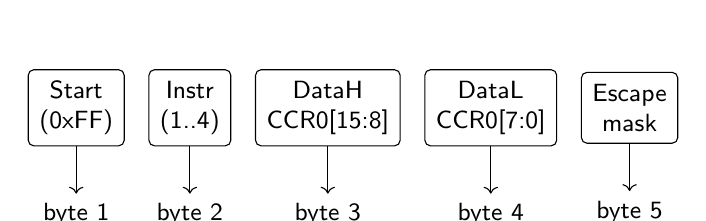
\begin{tikzpicture}[node distance=0.3cm, font=\sffamily\small]
    \tikzstyle{field}=[rectangle, draw, rounded corners=2pt, minimum height=0.9cm, align=center, inner sep=4pt]
    \node[field] (start) {Start\\(0xFF)};
    \node[field, right=of start] (instr) {Instr\\(1..4)};
    \node[field, right=of instr] (datah) {DataH\\CCR0[15:8]};
    \node[field, right=of datah] (datal) {DataL\\CCR0[7:0]};
    \node[field, right=of datal] (esc) {Escape\\mask};
    \draw[->] (start.south) -- ++(0,-0.6) node[below] {byte 1};
    \draw[->] (instr.south) -- ++(0,-0.6) node[below] {byte 2};
    \draw[->] (datah.south) -- ++(0,-0.6) node[below] {byte 3};
    \draw[->] (datal.south) -- ++(0,-0.6) node[below] {byte 4};
    \draw[->] (esc.south) -- ++(0,-0.6) node[below] {byte 5};
  \end{tikzpicture}
  \caption{UART packet layout for step/continuous commands}
  \label{fig:packet-diagram}
\end{figure}
\subsubsection{Communication Protocol}
The packet structure is designed for reliability. Table \ref{tab:packet} details the byte layout.

\begin{table}[H]
\centering
\begin{tabular}{|l|c|l|}
\hline
\textbf{Byte Name} & \textbf{Pos} & \textbf{Description} \\ \hline
Start Byte & 1 & Fixed at 255. synchronization marker. \\ \hline
Instruction Byte & 2 & \begin{tabular}[c]{@{}l@{}}1: CCW Continuous\\ 2: CW Continuous\\ 3/4: Single Step CCW/CW\end{tabular} \\ \hline
Data H & 3 & High byte of Timer CCR0 value (Speed Control) \\ \hline
Data L & 4 & Low byte of Timer CCR0 value \\ \hline
Escape Byte & 5 & \begin{tabular}[c]{@{}l@{}}Bitmask for handling 255 in data:\\ Bit 0: Data L was 255\\ Bit 1: Data H was 255\end{tabular} \\ \hline
\end{tabular}
\caption{UART Packet Structure}
\label{tab:packet}
\end{table}

Code snippet for packet building (from \texttt{StepperCommander.cs}):
\begin{lstlisting}[language=C, caption={Packet builder}, label={lst:build-packet}]
public byte[] BuildPacket(byte dirByte, ushort ccr0)
{
    byte high = (byte)(ccr0 >> 8);
    byte low = (byte)(ccr0 & 0xFF);
    byte escape = 0;
    // ... escape handling logic ...
    return new[] { StartByte, dirByte, high, low, escape };
}
\end{lstlisting}

\subsection{Results}

\begin{figure}[H]
\centering
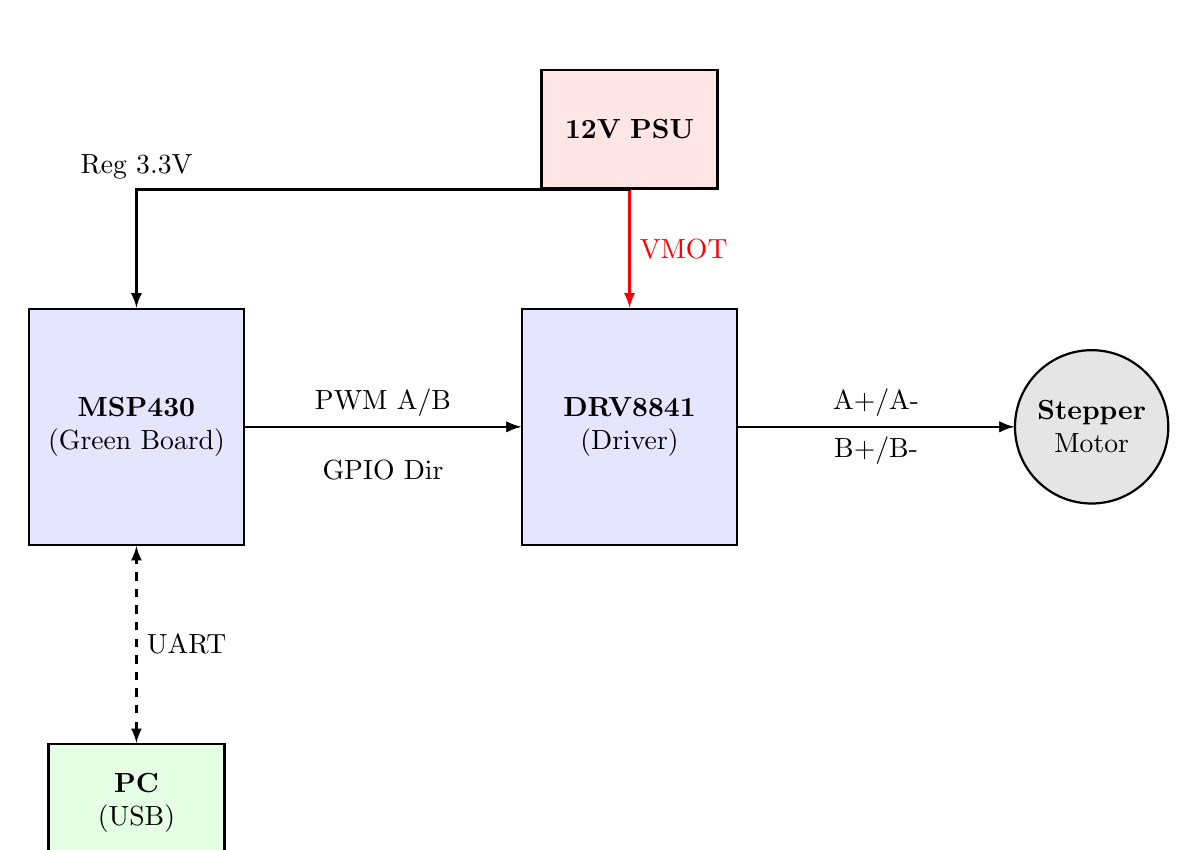
\begin{tikzpicture}[node distance=2.5cm, auto, >=latex, thick]
    % Styles
    \tikzstyle{block} = [rectangle, draw, fill=blue!10, text width=2.5cm, text centered, minimum height=3cm]
    \tikzstyle{motor} = [circle, draw, fill=gray!20, text width=1.5cm, text centered, minimum height=1.5cm]
    \tikzstyle{psu} = [rectangle, draw, fill=red!10, text width=2cm, text centered, minimum height=1.5cm]

    % Nodes
    \node [block] (mcu) {\textbf{MSP430}\\(Green Board)};
    \node [block, right=of mcu, xshift=1cm] (driver) {\textbf{DRV8841}\\(Driver)};
    \node [motor, right=of driver, xshift=1cm] (stepper) {\textbf{Stepper}\\Motor};
    \node [psu, above=of driver, yshift=-1cm] (power) {\textbf{12V PSU}};
    \node [psu, below=of mcu, fill=green!10] (pc) {\textbf{PC}\\(USB)};

    % Connections
    % Power
    \draw[->, red] (power.south) -- (driver.north) node[midway, right] {VMOT};
    \draw[->] (power.south) -| (mcu.north) node[midway, above] {Reg 3.3V};

    % Logic
    \draw[->] (mcu.east) -- (driver.west) node[midway, above] {PWM A/B};
    \draw[->] (mcu.east) -- (driver.west) node[midway, below, yshift=-0.3cm] {GPIO Dir};
    
    % Motor
    \draw[->] (driver.east) -- (stepper.west) node[midway, above] {A+/A-};
    \draw[->] (driver.east) -- (stepper.west) node[midway, below] {B+/B-};
    
    % PC
    \draw[<->, dashed] (pc.north) -- (mcu.south) node[midway, right] {UART};

\end{tikzpicture}
\caption{Electrical Schematic of Stepper Control System}
\label{fig:sch_ex2}
\end{figure}

The exact pin configuration is shown below

\begin{figure}[H]
\centering
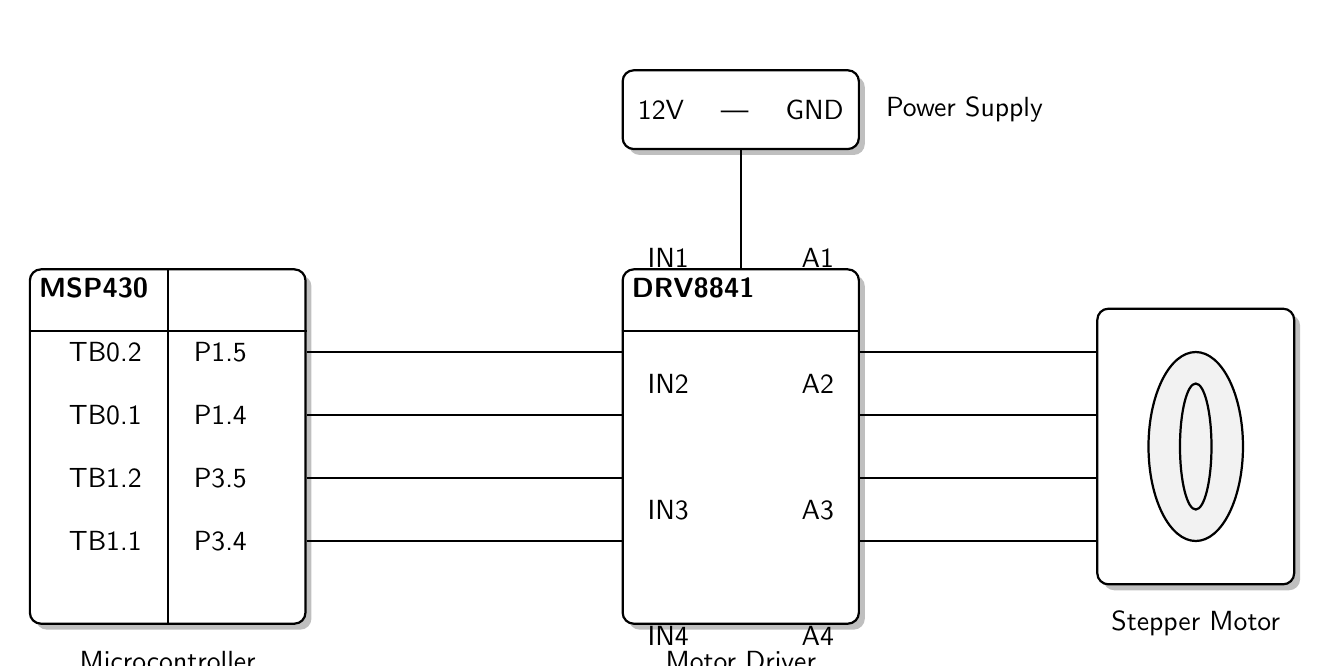
\begin{tikzpicture}[
    font=\sffamily,
    thick,
    component/.style={
        draw,
        rounded corners,
        fill=white,
        drop shadow,
        align=center,
        inner sep=5pt
    },
    wire/.style={
        thick
    }
]

% MSP430 Block
\node[component, minimum width=3.5cm, minimum height=4.5cm] (msp) at (0,0) {};
\node[anchor=north west] at (msp.north west) {\textbf{MSP430}};
\node[below=0.2cm] at (msp.south) {Microcontroller};

% Internal separator line
\draw ([yshift=-0.8cm]msp.north west) -- ([yshift=-0.8cm]msp.north east);
\draw (msp.north) -- (msp.south);

% Pin Labels
\foreach \tb/\p/\y/\i in {TB0.2/P1.5/1.2/1, TB0.1/P1.4/0.4/2, TB1.2/P3.5/-0.4/3, TB1.1/P3.4/-1.2/4} {
    \node[anchor=east] at ([xshift=-0.2cm, yshift=\y cm]msp.center) {\tb};
    \node[anchor=west] at ([xshift=0.2cm, yshift=\y cm]msp.center) {\p};
    \coordinate (msp_out_\i) at (msp.east |- 0, \y);
}


% DRV8841 Block
\node[component, minimum width=3cm, minimum height=4.5cm, right=4cm of msp] (drv) {};
\node[anchor=north west] at (drv.north west) {\textbf{DRV8841}};
\node[below=0.2cm] at (drv.south) {Motor Driver};

% Internal separator line
\draw ([yshift=-0.8cm]drv.north west) -- ([yshift=-0.8cm]drv.north east);

% DRV Pins
\foreach \in/\out/\y/\i in {IN1/A1/1.2/1, IN2/A2/0.4/2, IN3/A3/-0.4/3, IN4/A4/-1.2/4} {
    \node[anchor=west] at ([xshift=0.2cm, yshift=\y cm]drv.west |- 0, \y) {\in};
    \node[anchor=east] at ([xshift=-0.2cm, yshift=\y cm]drv.east |- 0, \y) {\out};
    \coordinate (drv_in_\i) at (drv.west |- 0, \y);
    \coordinate (drv_out_\i) at (drv.east |- 0, \y);
}


% Connections MSP -> DRV
\foreach \i in {1,2,3,4} {
    \draw (msp_out_\i) -- (drv_in_\i);
}


% Stepper Motor Block
\node[component, minimum width=2.5cm, minimum height=3.5cm, right=3cm of drv] (motor) {};
\node[below=0.2cm] at (motor.south) {Stepper Motor};

% Motor Symbol (Oval)
\draw[fill=gray!10] (motor.center) ellipse (0.6cm and 1.2cm);
\draw (motor.center) ellipse (0.2cm and 0.8cm); % Inner detail


% Connections DRV -> Motor
\foreach \i in {1,2,3,4} {
    \draw (drv_out_\i) -- (motor.west |- drv_out_\i);
}


% Power Supply Block
\node[component, minimum width=3cm, minimum height=1cm, above=1.5cm of drv] (power) {12V \quad | \quad GND};
\node[right=0.2cm] at (power.east) {Power Supply};

% Power Connections
\draw (power.south) -- (drv.north);

\end{tikzpicture}
\caption{Electrical Schematic of Stepper Control System}
\label{fig:sch_ex2}
\end{figure}


\subsection{Speed Results and Limits}
\textbf{Measured and commanded speeds:}
From our software, we are sending a maximum frequency of 1200 Hz. Since each pulse creates a half step, the value for theoretical step/s is
\begin{equation}
    f_{\text{steps}} = \frac{f_{\text{max}}}{2} = \frac{1200}{2} = 600 \text{ steps/s}
\end{equation}
For a motor with 200 steps/rev, this is
\begin{equation}
    \text{rev/s}_{\text{cmd}} = \frac{f_{\text{steps}}}{200} = \frac{600}{200} = 3 \text{ rev/s}
\end{equation}

We then measured the actual speed of the motor using the scope in \Cref{fig:motor_oscilloscope}. The scope captured a stable step frequency of $f_{\text{steps}} \approx 759$ Hz; 
which gives $\text{steps/s}_{\text{meas}} = \frac{759}{2} = 379.5 \text{ steps/s}$ and $\text{rev/s}_{\text{meas}}=\frac{759}{2*200}=1.895$ rev/s.

\begin{figure}[H]
    \centering
    \includegraphics[width=0.8\textwidth]{figures/motor_oscilloscope.png}
    \caption{Scope capture of step frequency}
    \label{fig:motor_oscilloscope}
\end{figure}

\subsubsection{Discussion}
The theoretical UI ceiling is fixed by $f_{\text{max}} = 1200$ Hz, corresponding to a shaft speed of 3 rev/s. However, our experimental results demonstrated a physical limit of approximately $1.9$ rev/s ($f_{\text{ISR}} \approx 759$ Hz) before the motor lost synchronization.

We think that this discrepancy is primarily governed by the physical properties of the motor. The Pololu 1208 stepper has a relatively high coil 
inductance ($13.5$ mH). As the step rate increases, the back-EMF rises and the time 
interval available to energize the coils decreases, preventing the current from reaching its rated level. This results in a sharp torque reduction, causing the motor to stall well below the software limit.

Additionally, software timing errors may contribute to the restricted speed. At higher frequencies, interrupt latency or timing jitter can introduce uneven step intervals. This instability can cause the motor to stall prematurely by momentarily demanding a higher acceleration than the available torque can support. Practically, a safe operating ceiling should be set near 1.5 rev/s to account for these physical and timing variances.

\subsection{Challenges}
\begin{enumerate}
    \item Connecting the stepper motor coils (A1, A2, B1, B2) to the driver required careful verification. Swapping a pair could reverse direction or cause vibration without movement.
    \item Setting the VREF on the driver was critical. If too low, the motor skips steps; if too high, the motor/driver overheats.
    \item Starting the motor at high speed immediately causes stalling due to inertia. We had to find the maximum start speed to avoid this.
    \item At certain speeds, the motor vibrates excessively. Avoiding those specific frequencies helped maintain smooth operation.
    \item Sending commands too fast from the PC caused the RX buffer to overflow. Implementing a circular buffer fixed this issue.
\end{enumerate}

\section{Exercise 3: 2-Axis Control with Dual Stepper Motors}

\subsection{Objective}
To extend the system to 2 axes (X and Y) for a gantry stage. This requires driving a second stepper motor using an external H-bridge driver wired to the PCB.

\subsection{Procedure}

\subsubsection{Gantry Assembly}
The 2-axis gantry was assembled using V-slot aluminum extrusions and timing belts. The procedure followed the standard build provided in the lab manual, with the following key steps:
\begin{enumerate}
    \item \textbf{Frame}: Assembled the base frame using corner brackets and T-nuts.
    \item \textbf{X-Axis}: Mounted the X-axis carriage and belt drive.
    \item \textbf{Y-Axis}: Mounted the Y-axis extrusion on top of the X-carriage.
    \item \textbf{Pen Holder}:  We designed and 3D printed a custom pen holder that attaches to the Y-axis slider. This holder uses a interference fit to secure a Sharpie marker, ensuring rigid contact with the paper during drawing operations.
\end{enumerate}
Our assembled gantry is shown in Figure \ref{fig:gantry}.

\begin{figure}[H]
  \centering
  \includegraphics[width=0.8\textwidth]{figures/gantry_annotated.jpg}%
  \caption{Gantry Assembly}
  \label{fig:gantry}
\end{figure}

\subsubsection{Motor 2 Pin Map and Wiring Reference}
Motor 1 (X) uses the same wiring diagram for part 2 with timer PWM pins (TB0.1/0.2 on P1.4/P1.5 and TB1.1/1.2 on P3.4/P3.5). 
For Motor 2 (Y), we need to use the external driver which uses the GPIO-mapped driver pins below:
\begin{itemize}
    \item P1.3 $\rightarrow$ Motor 2 PWM/enable
    \item PJ.0/PJ.1 $\rightarrow$ AIN2/AIN1 (Coil A)
    \item PJ.2/PJ.3 $\rightarrow$ BIN1/BIN2 (Coil B)
\end{itemize}

\begin{figure}[H]
  \centering
  \includegraphics[width=0.8\textwidth]{figures/ex3_wiring_diagram.png}
  \caption{2-axis control wiring diagram}
  \label{fig:ex3-wiring}
\end{figure}

\subsubsection{Coordinated Motion Control (Firmware)}
The firmware implements a Bresenham-like DDA (Digital Differential Analyzer) algorithm to drive both motors simultaneously in a straight line. The `start\_move` function calculates the total steps needed (the larger of $\Delta x$ or $\Delta y$) and sets the timer frequency based on the requested speed.

The firmware receives an 8-byte packet from the PC to initiate moves. The packet structure is shown in Figure \ref{fig:ex3-packet}.

\begin{figure}[H]
  \centering
  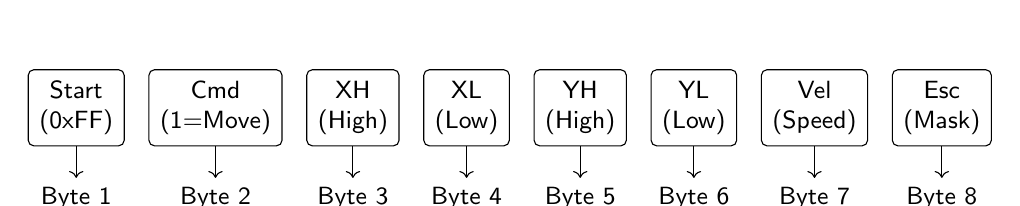
\begin{tikzpicture}[node distance=0.3cm, font=\sffamily\small]
    \tikzstyle{field}=[rectangle, draw, rounded corners=2pt, minimum height=0.9cm, align=center, inner sep=4pt]
    \node[field] (start) {Start\\(0xFF)};
    \node[field, right=of start] (cmd) {Cmd\\(1=Move)};
    \node[field, right=of cmd] (xh) {XH\\(High)};
    \node[field, right=of xh] (xl) {XL\\(Low)};
    \node[field, right=of xl] (yh) {YH\\(High)};
    \node[field, right=of yh] (yl) {YL\\(Low)};
    \node[field, right=of yl] (vel) {Vel\\(Speed)};
    \node[field, right=of vel] (esc) {Esc\\(Mask)};
    
    \draw[->] (start.south) -- ++(0,-0.4) node[below] {Byte 1};
    \draw[->] (cmd.south) -- ++(0,-0.4) node[below] {Byte 2};
    \draw[->] (xh.south) -- ++(0,-0.4) node[below] {Byte 3};
    \draw[->] (xl.south) -- ++(0,-0.4) node[below] {Byte 4};
    \draw[->] (yh.south) -- ++(0,-0.4) node[below] {Byte 5};
    \draw[->] (yl.south) -- ++(0,-0.4) node[below] {Byte 6};
    \draw[->] (vel.south) -- ++(0,-0.4) node[below] {Byte 7};
    \draw[->] (esc.south) -- ++(0,-0.4) node[below] {Byte 8};
  \end{tikzpicture}
  \caption{UART packet structure for 2-axis control (8 bytes)}
  \label{fig:ex3-packet}
\end{figure}

\begin{lstlisting}[language=C, caption={Firmware: Start Move Logic}, label={lst:start-move}]
void start_move(int16_t dx, int16_t dy, uint8_t speed) {
    delta_x = abs(dx);
    delta_y = abs(dy);
    total_steps_needed = (delta_x > delta_y) ? delta_x : delta_y;
    
    // Speed mapping: CCR0 = 40000 / speed
    if (speed == 0) speed = 1;
    TA1CCR0 = 40000 / speed; 

    is_moving = 1;
    TA1CTL |= MC__UP; // Start Timer
}
\end{lstlisting}

The Timer A1 ISR executes the stepping logic. It accumulates the delta values and steps the respective motor when the accumulator exceeds the total steps. This ensures the slope is maintained.

\begin{lstlisting}[language=C, caption={Firmware: DDA Stepping ISR}, label={lst:dda-isr}]
__interrupt void Timer_A1_ISR(void) {
    acc_x += delta_x;
    acc_y += delta_y;

    if (acc_x >= total_steps_needed) {
        motor1_state = (motor1_state + step_x_inc) & 0x07;
        step_motor1(motor1_state);
        acc_x -= total_steps_needed;
    }
    
    if (acc_y >= total_steps_needed) {
        motor2_state = (motor2_state + step_y_inc) & 0x07;
        step_motor2(motor2_state);
        acc_y -= total_steps_needed;
    }
}
\end{lstlisting}

To control the gantry, we use C\# to create a simple UI to control the gantry. there are 3 specifics features:
\begin{itemize}
    \item Manual Move Control
    \item Continuous Move Control
    \item Image Processing
\end{itemize}

\subsection{Feature 1: Manual Move Control}
The first feature allows us to move the gantry by a specific relative distance in X and Y.
We can also set the speed of each gantry axis.

\subsubsection{Software Implementation}
The C\# application takes input in centimeters and converts it to steps. The linear movement depends on the bore of the pulley,
from our calibration we found that for our system, the steps per cm is:
\begin{itemize}
    \item Motor 1 (UI Y): 100 steps/cm
    \item Motor 2 (UI X): 125 steps/cm
\end{itemize}
\[
dx_{\text{steps}} = y_{\text{cm}} \times 100, \quad dy_{\text{steps}} = x_{\text{cm}} \times 125
\]
The velocity slider (1-100\%) is mapped to a firmware speed byte (1-6) to limit the maximum speed to a safe range.

\begin{lstlisting}[language=C, caption={Software: Manual Move Command}, label={lst:move-btn}]
private void MoveBtn_Click(object sender, RoutedEventArgs e)
{
    // Axis Flip: UI X -> Motor 2, UI Y -> Motor 1
    int dx = (int)(yCm * STEPS_PER_CM_M1); 
    int dy = (int)(xCm * STEPS_PER_CM_M2);
    
    // Speed Mapping
    double targetMax = 1.0 + (50.0 - 1.0) * 11.0 / 99.0; // ~6.44
    int actualSpeed = (int)Math.Round(1.0 + (uiSpeed - 1.0) * (targetMax - 1.0) / 99.0);
    
    SendPacket(dx, dy, actualSpeed);
}
\end{lstlisting}

\begin{figure}[H]
  \centering
  \includegraphics[width=0.8\textwidth]{figures/ex_3_move.png}
  \caption{Manual Move UI}
  \label{fig:ex3-move}
\end{figure}

\subsubsection{Results}
Using this feature, we can move the gantry to any position in the workspace. We used this to test our test drawing as instructed by the Lab Manual, where we moved as follows:

\begin{table}[H]
\centering
\begin{tabular}{|c|c|c|c|}
\hline
\textbf{Location} & \textbf{X (cm)} & \textbf{Y (cm)} & \textbf{Velocity (\%)} \\ \hline
1 & 5 & 0 & 100 \\ \hline
2 & 0 & 5 & 50 \\ \hline
3 & -5 & -5 & 20 \\ \hline
4 & 7 & 2 & 60 \\ \hline
5 & -7 & 3 & 80 \\ \hline
6 & 0 & -5 & 10 \\ \hline
\end{tabular}
\caption{Test Move Sequence}
\label{tab:test-moves}
\end{table}

The simulated path of these relative moves is shown below. Starting from $(0,0)$, the gantry visits points $(5,0) \rightarrow (5,5) \rightarrow (0,0) \rightarrow (7,2) \rightarrow (0,5) \rightarrow (0,0)$.

\begin{figure}[H]
  \centering
  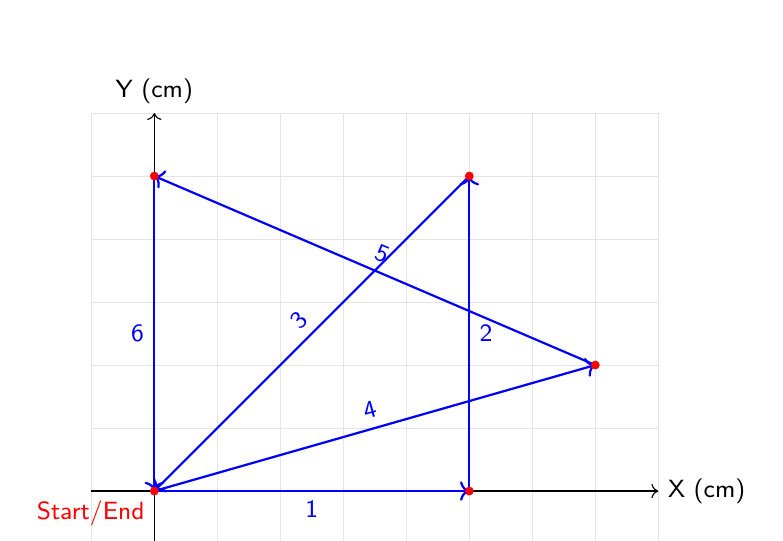
\begin{tikzpicture}[scale=0.8, font=\sffamily\small]
    % Grid
    \draw[step=1cm, gray!20, very thin] (-1,-1) grid (8,6);
    \draw[->] (-1,0) -- (8,0) node[right] {X (cm)};
    \draw[->] (0,-1) -- (0,6) node[above] {Y (cm)};
    
    % Path
    \coordinate (p0) at (0,0);
    \coordinate (p1) at (5,0);
    \coordinate (p2) at (5,5);
    \coordinate (p3) at (0,0);
    \coordinate (p4) at (7,2);
    \coordinate (p5) at (0,5);
    \coordinate (p6) at (0,0);
    
    \draw[thick, blue, ->] (p0) -- (p1) node[midway, below] {1};
    \draw[thick, blue, ->] (p1) -- (p2) node[midway, right] {2};
    \draw[thick, blue, ->] (p2) -- (p3) node[midway, sloped, above] {3};
    \draw[thick, blue, ->] (p3) -- (p4) node[midway, sloped, above] {4};
    \draw[thick, blue, ->] (p4) -- (p5) node[midway, sloped, above] {5};
    \draw[thick, blue, ->] (p5) -- (p6) node[midway, left] {6};
    
    % Points
    \fill[red] (p0) circle (2pt) node[below left] {Start/End};
    \fill[red] (p1) circle (2pt);
    \fill[red] (p2) circle (2pt);
    \fill[red] (p4) circle (2pt);
    \fill[red] (p5) circle (2pt);
    
  \end{tikzpicture}
  \caption{Simulated Path of Test Moves}
  \label{fig:sim-path}
\end{figure}

The resulting picture can be seen below

\begin{figure}[H]
  \centering
  \includegraphics[width=0.8\textwidth]{figures/ex3_part1_result.jpg}
  \caption{Lab movement result}
  \label{fig:ex3-move}
\end{figure}
Note that the picture has a lot of red colored marks due to the bleeding of the red marker as well as because we were 
trying to draw another picture after it has successfully finished drawing the first picture. However, the shape of the
picture is still recognizable and the TA has already confirmed that the picture is correct.

\subsection{Feature 2: Canvas Drawing}
This feature allows the user to draw on a digital canvas, which is then replicated by the gantry.

\subsubsection{Software Implementation}
The drawing is captured as a bitmap. The software iterates through pixels, identifying dark pixels as points to draw. These points are mapped from pixel coordinates to physical centimeters.

\textbf{Coordinate Mapping:}
The canvas is 300x300 pixels, mapped to a 12x12 cm area centered at (0,0).
\[
X_{\text{cm}} = \left(\frac{x_{\text{px}}}{W} \times 12\right) - 6, \quad Y_{\text{cm}} = -\left[\left(\frac{y_{\text{px}}}{H} \times 12\right) - 6\right]
\]

To optimize movement, points are sorted using a Nearest Neighbor algorithm to minimize travel distance between points.

\begin{lstlisting}[language=C, caption={Software: Nearest Neighbor Sorting}, label={lst:nearest-neighbor}]
private List<Point> SortPointsNearestNeighbor(List<Point> points)
{
    List<Point> sorted = new List<Point>();
    Point current = new Point(_currentX, _currentY);
    
    while (sorted.Count < points.Count) {
        // Find point with min distance squared to current
        double minDistSq = double.MaxValue;
        // ... (Loop through points) ...
        // dSq = (p.X - c.X)^2 + (p.Y - c.Y)^2
    }
    return sorted;
}
\end{lstlisting}

\begin{figure}[H]
  \centering
  \begin{subfigure}[b]{0.45\textwidth}
    \includegraphics[width=\textwidth]{figures/ex_3_creative_square.png}
    \caption{Square Drawing}
  \end{subfigure}
  \hfill
  \begin{subfigure}[b]{0.45\textwidth}
    \includegraphics[width=\textwidth]{figures/ex_3_creative_star.png}
    \caption{Star Drawing}
  \end{subfigure}
  \caption{Canvas Drawing Examples}
  \label{fig:ex3-drawing}
\end{figure}

\subsubsection{Results}
When we tried to draw the star in \Cref{fig:ex3-drawing}, the result is shown in \Cref{fig:ex3-drawing-star}. 
The gantry was able to trace the star shape using a series of triangle due to the nature of the closest neighbor algorithm. 
But, since the bed is not properly leveled, some part of the marker did not touch the bed, hence the missing triangle (marked in blue)
that was later added on by the TA by retracing it's path. That is, the motion planning was good and works as expected.
\begin{figure}[H]
  \centering
  \includegraphics[width=0.8\textwidth]{figures/ex3_freeform_star_result.jpg}
  \caption{Star Drawing Result}
  \label{fig:ex3-drawing-star}
\end{figure}

\subsection{Feature 3: Image to Bitmap (Edge Detection)}
The final feature imports an image, detects edges, and converts them into a drawing path.

\subsubsection{Software Implementation}
The core of this feature is the Sobel edge detection algorithm, which identifies boundaries within an image by calculating the gradient of image intensity at each pixel.

\textbf{1. Grayscale Conversion:}
First, the input image is converted to an 8-bit grayscale format, where each pixel $P(x,y)$ represents an intensity value from 0 (black) to 255 (white).

\textbf{2. Convolution with Sobel Kernels:}
We apply two $3\times3$ convolution kernels, $G_x$ and $G_y$, to the image. $G_x$ detects horizontal changes (vertical edges), and $G_y$ detects vertical changes (horizontal edges).

\[
G_x = \begin{bmatrix} -1 & 0 & 1 \\ -2 & 0 & 2 \\ -1 & 0 & 1 \end{bmatrix}, \quad
G_y = \begin{bmatrix} -1 & -2 & -1 \\ 0 & 0 & 0 \\ 1 & 2 & 1 \end{bmatrix}
\]

For a pixel at $(x,y)$, the horizontal gradient approximation $g_x$ is computed by convolving the neighborhood with $G_x$:
\begin{align*}
g_x &= -P(x-1, y-1) + P(x+1, y-1) \\
    &\quad -2P(x-1, y) + 2P(x+1, y) \\
    &\quad -P(x-1, y+1) + P(x+1, y+1)
\end{align*}
Similarly, $g_y$ is computed using $G_y$.

\textbf{3. Gradient Magnitude:}
The total gradient magnitude $G$ for the pixel is calculated as the Euclidean distance of the gradient vector:
\[
G = \sqrt{g_x^2 + g_y^2}
\]
This magnitude represents the strength of the edge at that pixel.

\textbf{4. Thresholding:}
To create a binary "edge map," we compare $G$ against a user-defined threshold $T$.
\[
\text{Edge}(x,y) = \begin{cases} 
255 (\text{White}) & \text{if } G > T \\
0 (\text{Black}) & \text{otherwise}
\end{cases}
\]

\begin{lstlisting}[language=C, caption={Software: Sobel Edge Detection Loop}, label={lst:sobel}]
// Iterate through image pixels (excluding border)
for (int y = 1; y < height - 1; y++) {
    for (int x = 1; x < width - 1; x++) {
        // Compute gx and gy using the kernels
        int gx = ...; 
        int gy = ...;

        int mag = (int)Math.Sqrt(gx * gx + gy * gy);
        
        // Thresholding
        resultPixels[i] = (byte)(mag > threshold ? 255 : 0);
    }
}
\end{lstlisting}

The resulting binary image is then processed to extract the coordinates of all white pixels. These points are sorted using the Nearest Neighbor algorithm to form a continuous drawing path for the gantry.

\subsubsection{Results}
The following images show the results of the image processing. We traced a drawing from a comic book character in My Hero Academia, called 
Deku. The result is shown in \Cref{fig:ex3-deku}. Since there is not much edges and background, this image shows a good example of a drawable image for our gantry.

\begin{figure}[H]
  \centering
  \begin{subfigure}[b]{0.45\textwidth}
    \includegraphics[width=\textwidth]{figures/ex3_image_deku.png}
    \caption{Original Image (Deku)}
  \end{subfigure}
  \hfill
  \begin{subfigure}[b]{0.45\textwidth}
    \includegraphics[width=\textwidth]{figures/ex3_image_deku_converted.png}
    \caption{Edge Detected}
  \end{subfigure}
  \caption{Image Processing Example 1}
  \label{fig:ex3-deku}
\end{figure}

On the other hand, when we tried to draw Prof. Hong Ma, the present of multiple object in the background made it hard to trace the edges.

\begin{figure}[H]
  \centering
  \begin{subfigure}[b]{0.45\textwidth}
    \includegraphics[width=\textwidth]{figures/ex3_image_hong.png}
    \caption{Original Image (Hong)}
  \end{subfigure}
  \hfill
  \begin{subfigure}[b]{0.45\textwidth}
    \includegraphics[width=\textwidth]{figures/ex3_image_hong_converted.png}
    \caption{Edge Detected}
  \end{subfigure}
  \caption{Image Processing Example 2}
  \label{fig:ex3-hong}
\end{figure}

When we tried to draw Deku however, the result was not as expected. The image was too complex and perhaps it required more advanced path planning or 
resolution. The result is shown in \Cref{fig:ex3-deku-drawing}. 

\begin{figure}[H]
  \centering
  \includegraphics[width=0.8\textwidth]{figures/ex3_deku_result.jpg}
  \caption{Drawing Result (Deku)}
  \label{fig:ex3-deku-drawing}
\end{figure}
This is most likely because after drawing the fist, the gantry tries to draw the face, however since it requires point skipping, 
the gantry is unable to draw the face. This coupled with the fact that we did not have a Z-axis, control for the height of the marker, 
means that even if we were able to plan the path, the gantry would not be able to draw the face eitherway. Regardless, it is still a fun exercise
for turning the images into a bitmap for drawing.

\subsection{Discussion: Stepper Motor Performance}
Stepper motors offer distinct advantages for 2-axis stage control, primarily their ability to provide precise open-loop position control without the need for encoders. This simplifies the control architecture significantly. They also provide high holding torque, which ensures the gantry maintains its position when stationary. The digital interface (step and direction signals) is straightforward to implement with microcontrollers.

However, there are limitations. Stepper motors are susceptible to resonance at specific speeds, which can cause vibration and noise. Since the system is open-loop, any skipped steps due to high load or acceleration result in permanent position errors for the remainder of the operation. Additionally, the discrete nature of stepping can cause "aliasing" or stair-stepping artifacts when drawing diagonal lines or curves, especially at low resolutions.

\textbf{Shape Difficulty Analysis:}
\begin{itemize}
    \item \textbf{Easy Shapes}: Straight lines, squares, and rectangles are the easiest to draw. They align well with the linear interpolation (DDA) algorithm and the orthogonal axes of the gantry. The motion is continuous and requires minimal acceleration changes.
    \item \textbf{Hard Shapes}: Circles, arcs, and complex curves are difficult. They must be approximated by a series of very short line segments. This requires the motor to constantly accelerate and decelerate, increasing the risk of vibration and step loss. The "stair-stepping" effect is also most visible on these shapes, requiring microstepping or higher gear reduction to smooth out.
\end{itemize}

\subsection{Challenges}
\begin{enumerate}
    \item The gantry rails were not perfectly parallel, causing binding at certain spots. We had to adjust the eccentric spacers and belt tension to ensure smooth movement.
    \item The assembly instructions was not consistent between each steps, thus we sometimes had to back track and reassemble the gantry.
    \item The belt has to be tightened to ensure smooth movement, otherwise the motor would skip, a friends suggested using a nut tightener like in 3D printers to help mitigate this.
    \item Converting pixel coordinates (0-300) to physical cm (-6 to 6) required careful calibration. We also had to flip the Y-axis in software to match the physical gantry orientation.
    \item Hysteresis in the belt drive caused circles to look like ovals. We minimized this by tightening the belts and ensuring the pulleys were secure.
    \item The lack of a Z-axis meant the pen dragged during "non-drawing" moves. We had to manually lift it or plan paths to minimize travel over the drawing area.
    \item The Sobel filter picked up too many edges from noisy images. Tuning the threshold was critical to get a clean drawing.
    \item Implementing the Bresenham/DDA algorithm for integer-based coordinated motion was challenging. We had to ensure no floating-point math was used in the ISR for performance.
    \item The marker would dry out if left uncapped or if the drawing took too long. We had to cap it between tests.
    \item At high speeds, the gantry wobble made wavy lines. Slowing down the drawing speed improved the quality significantly.
    \item The edge detection algorithm is good, however the actual drawing is very hard to replicate lightly because nearest neighbor causes
    very high point for image drawing. This causes it to twitch around and thus the results is not very good.
\end{enumerate}

\section{Conclusion}
This lab successfully demonstrated the complete process of building a mechatronic controller, from soldering the PCB to implementing low-level motor control firmware and high-level PC software. The final 2-axis gantry system was able to draw complex shapes, validating the integration of all subsystems.

\newpage
\newpage
\appendix
\section{Exercise 2 Code}
\subsection{Microcontroller Firmware}
\lstinputlisting[language=C, caption=Microcontroller Firmware (Ex2)]{code/ex2/main.c}

\subsection{PC Interface (C\#)}
\lstinputlisting[language=C, caption=StepperCommander.cs]{code/ex2/StepperCommander.cs}
\lstinputlisting[language=C, caption=Form1.cs]{code/ex2/Form1.cs}

\section{Exercise 3 Code}
\subsection{Microcontroller Firmware}
\lstinputlisting[language=C, caption=main.c]{code/ex3/main.c}

\subsection{PC Interface (C\#)}
\lstinputlisting[language=C, caption=MainWindow.xaml.cs]{code/ex3/MainWindow.xaml.cs}

\section{Gantry Assembly}
\textbf{Safety}: Please note there are a number of risks to be aware of while working with this device. Ensure the device is on a stable and level surface before operating. Keep fingers, hair, and loose clothing away from the device when it is operational. Keep your hands and any liquids away from the electronics while the circuit is live, only ever work on the circuit when it is not powered or plugged into a power source.

\subsection*{Step 1. Assemble the Frame}
\begin{enumerate}
    \item Gather the necessary components.
    \item Mount one side of the X-axis beam, put the slider on the extrusion.
    \item Mount the other side of the X-axis beam.
    \item Flip the base, and place the other two extrusions as shown.
    \item Fix the four corners.
    \item The base should now look like this.
    \item Gather the necessary components for the top of the frame.
    \item Mount the two support arms, front and back.
    \item Mount the Y-axis beam with the slider on the extrusion.
\end{enumerate}

\subsection*{Step 2. Assemble the X-axis}
\begin{enumerate}
    \item Gather necessary components.
    \item Mount the free pulley.
    \item Mount the DC motor mount.
    \item Gather DC motor parts. \textit{Note: DC motor in photo has been upgraded.}
    \item Mount the DC motor.
    \item Attach the 4mm bore gear.
\end{enumerate}

\subsection*{Step 3. Assemble the Y-axis}
\begin{enumerate}
    \item Gather necessary components. \textit{Note: Stepper motor in photo has been upgraded.}
    \item Mount the components similar to the X-axis. \textit{Note: Stepper motor mounted with nuts and bolts.}
    \item \textbf{Custom Marker Holder}: We designed and CADed a custom marker holder which mounts onto the gantry Y-axis slider. The holder features a press-fit mechanism to securely hold the marker during operation.
\end{enumerate}

\subsection*{Step 4. Assembling the belt drive}
\begin{enumerate}
    \item Feed belt through V-slot extrusion.
    \item Loop through slider. \textit{Note: Timing belt should lock with itself.}
    \item Zip tie the timing belt together.
    \item Zip tie the other end. \textit{Note: Timing belt should be looped around both the gear and free pulley.}
    \item Tighten the belt at the free pulley end.
    \item Repeat on the Y-axis.
\end{enumerate}

\section{Appendix D: PCB Photos}
\begin{figure}[H]
    \centering
    \includegraphics[width=0.8\textwidth]{figures/pcb_board_front_appendix_1.jpeg}
    \caption{PCB Front View 1}
\end{figure}
\begin{figure}[H]
    \centering
    \includegraphics[width=0.8\textwidth]{figures/pcb_board_front_appendix_2.jpeg}
    \caption{PCB Front View 2}
\end{figure}
\begin{figure}[H]
    \centering
    \includegraphics[width=0.8\textwidth]{figures/pcb_board_front_appendix_3.jpeg}
    \caption{PCB Front View 3}
\end{figure}
\begin{figure}[H]
    \centering
    \includegraphics[width=0.8\textwidth]{figures/pcb_board_front_appendix_4.jpeg}
    \caption{PCB Front View 4}
\end{figure}
\begin{figure}[H]
    \centering
    \includegraphics[width=0.8\textwidth]{figures/pcb_board_front_appendix_5.jpeg}
    \caption{PCB Front View 5}
\end{figure}
\begin{figure}[H]
    \centering
    \includegraphics[width=0.8\textwidth]{figures/pcb_board_front_appendix_6.jpeg}
    \caption{PCB Front View 6}
\end{figure}
\begin{figure}[H]
    \centering
    \includegraphics[width=0.8\textwidth]{figures/pcb_board_front_appendix_7.jpeg}
    \caption{PCB Front View 7}
\end{figure}

\end{document}
